% !TeX document-id = {075bf025-0d99-414a-b21e-a2ac906020fb}
% !TeX encoding = UTF-8
% !TeX program = pdflatex
% !BIB program = biber
% Template Revision:
% Rev. A2 -- 2019-11-04 -- A. Varli
% Rev. B1 -- 2019-11-05 -- A. Varli
%% HINWEISE:
%% MAIN.tex ist die Hauptdatei. Hier sind sämtliche Pakete eingebunden und die allgemeine Struktur ist hier festgelegt. Im Allgemeinen müssen hier keine Änderungen vorgenommen werden.
%% In der eingebundenen Datei config.tex müssen Änderungen vorgenommen werden, die in der Datei näher erläutert sind.
%% Das Deckblatt wird mit der Datei cover/coversheet.tex eingebunden. Hier sollten keine Änderungen vorgenommen werden.
%% Für Text im Vorspann (vor der Inhaltsangabe, z.B. für Vorwort, Abstract etc.) ist die Datei frontmatter.tex vorgesehen.
%% Für den Hauptteil ist die Datei mainmatter.tex vorgesehen.
%% Das Literaturverzeichnis ist die eingebundene Datei literature.bib.
%% Für Verbesserungsvorschläge bin ich gerne offen.
%% Viel Erfolg :). Linz, im Oktober 2019, Ali Varli, a_v@gmx.net.
%% PLEASE NOTE:
%% MAIN.tex is the main file. All packages are pooled here and the general structure is defined here. In general, no changes need to be made here.
%% Changes must be made in the included file config.tex. Detailed information is in the file.
%% The cover page is included with the file cover/coversheet.tex. No changes should be made here.
%% The file frontmatter.tex is provided for text in the lead text (before the summary, i.e. for the foreword, abstract, etc.).
%% The file mainmatter.tex is intended for the main part.
%% The bibliography is the included file literature.bib.
%% I am open to suggestions for improvement.
%% Good luck :-). Linz, October 2019, Ali Varli, a_v@gmx.net.
\documentclass[
		a4paper,
		oneside,
		onecolumn,
		openany,
		parskip=half*,
%		toc=flat,
%		chapterentrydots=true,
		table,
		11pt,
		fleqn,
%		draft
	]{scrbook}
	
	\usepackage[utf8]{inputenc}

	\input{config}
	
	\usepackage[T1]{fontenc}
	\usepackage{roboto}
	\usepackage{mathpazo}
	    
	\ifeng	\usepackage[ngerman,english]{babel}
	\else	\usepackage[english,ngerman]{babel}	
	\fi
		
	\usepackage{amsmath}
	\usepackage{siunitx}	

%% Zitierweise numerisch, Literaturverzeichnis alphabetisch sortiert:
%% Citation listed numerically, bibliography listed alphabetically:
	\usepackage[backend=biber,sortlocale=auto,style=numeric-comp]{biblatex}
%% Zitierweise numerisch, Literaturverzeichnis unsortiert:
%% Citation listed numerically, bibliography unsorted:
%	\usepackage[backend=biber,sorting=none,style=numeric-comp]{biblatex}
%% Zitierweise Autor-Jahr, Literaturverzeichnis alphabetisch sortiert:
%% Citation listed by author-year, bibliography listed alphabetically:
%	\usepackage[backend=biber,style=authoryear,bibstyle=authoryear,citestyle=authoryear,maxcitenames=2]{biblatex}
	\addbibresource{literature.bib}
    \usepackage{csquotes}
    
    \usepackage[a4paper,left=30mm,right=14mm,top=27mm,bottom=10mm,includeheadfoot]{geometry}

	\usepackage{lastpage}
	\usepackage{scrlayer-scrpage}
	\pagestyle{scrheadings}
	\clearscrheadfoot
	\ifeng	\ohead*{\includegraphics[width=3cm]{cover/jkuen.png}}
	\else	\ohead*{\includegraphics[width=3cm]{cover/jkude.png}}
	\fi
	\ifoot*{\date}
	\cfoot*{\name}
	\ofoot*{\pagemark/\pageref{LastPage}}	
	\setkomafont{pageheadfoot}{\sffamily \scriptsize}
	\setkomafont{pagenumber}{\sffamily \scriptsize}

	\usepackage[onehalfspacing]{setspace}
	
	\usepackage{pdfpages}

	\usepackage{tabularx}
	\usepackage{ltxtable}
	\usepackage{booktabs}
	\usepackage{rotating}
	\usepackage{colortbl}
	\usepackage{multirow}
	\usepackage{adjustbox}
	
	\usepackage{xcolor}

	\usepackage{graphicx}
	\usepackage{wrapfig}

	\usepackage[section]{placeins} %\FloatBarrier

	\usepackage{float} %[H]

	\usepackage{enumitem}
		
	\usepackage{subfiles}
	
	\usepackage{listings}
	
%	\usepackage[toc,lof,lot]{multitoc}

%	\usepackage[
%		bookmarksnumbered=true,
%		pdfborder={0 0 0},
%		pdfa,
%		pdftitle={\pdfTitle},
%		pdfauthor={\pdfAuthor},
%		pdfsubject={\pdfSubject},
%		pdfkeywords={\pdfKeywords}]{hyperref}
	
%	\setcounter{tocdepth}{3} %subsubsection
%	\setcounter{secnumdepth}{3}
		
	\tolerance=100
	\clubpenalty=10000
	\widowpenalty=10000
	\displaywidowpenalty=10000
	
%	\addtocontents{toc}{\protect\enlargethispage{2\normalbaselineskip}}
%	\addtocontents{lof}{\protect\enlargethispage{2\normalbaselineskip}}
%	\addtocontents{lot}{\protect\enlargethispage{2\normalbaselineskip}}
	
	\addtokomafont{caption}{\small}
	\setkomafont{captionlabel}{\small\sffamily\bfseries}
	
	
	% own shit
	\usepackage{color}
	\definecolor{lightgray}{rgb}{.9,.9,.9}
	\definecolor{darkgray}{rgb}{.4,.4,.4}
	\definecolor{purple}{rgb}{0.65, 0.12, 0.82}
	\definecolor{lightorange}{rgb}{1,0.63,0}
	\definecolor{lightgreen}{rgb}{0,1,0.63}
	\definecolor{lightblue}{rgb}{0.31,0.63,1}
	
	\lstdefinelanguage{JavaScript}{
		keywords={typeof, new, true, false, catch, function, return, null, catch, switch, var, if, in, while, do, else, case, break},
		keywordstyle=\color{blue}\bfseries,
		ndkeywords={class, export, boolean, throw, implements, import, this},
		ndkeywordstyle=\color{darkgray}\bfseries,
		identifierstyle=\color{black},
		sensitive=false,
		comment=[l]{//},
		morecomment=[s]{/*}{*/},
		commentstyle=\color{purple}\ttfamily,
		stringstyle=\color{red}\ttfamily,
		morestring=[b]',
		morestring=[b]"
	}
	
	\lstset{
		language=JavaScript,
		backgroundcolor=\color{lightgray},
		extendedchars=true,
		basicstyle=\footnotesize\ttfamily,
		showstringspaces=false,
		showspaces=false,
		numbers=left,
		numberstyle=\footnotesize,
		numbersep=9pt,
		tabsize=2,
		breaklines=true,
		showtabs=false,
		captionpos=b
	}

%\usepackage{tikz}
%\usetikzlibrary{positioning}
%\usetikzlibrary{graphdrawing.trees}
%
%%
%%%%
%%%%%%%%
%%%%%%%%%%%%%%%%
\begin{document}
%%%%%%%%%%%%%%%%

\begin{titlepage}
\include{cover/coversheet}
\end{titlepage}


%%%%%%%%%%%%
\frontmatter

% !TeX encoding = UTF-8
% !TeX root = MAIN.tex

	\ifeng \chapter*{Sworn Declaration}
	I hereby declare under oath that the submitted thesis has been written solely by me without any third-party assistance, information other than provided sources or aids have not been used and those used have been fully documented. Sources for literal, paraphrased and cited quotes have been accurately credited.
	
	The submitted document here present is identical to the electronically submitted text document.
	
	\vskip1cm
	\place, \date
	
	\else \chapter*{Eidesstattliche Erklärung}
	Ich erkläre an Eides statt, dass ich die vorliegende Arbeit selbstständig und ohne fremde Hilfe verfasst, andere als die angegebenen Quellen und Hilfsmittel nicht benutzt bzw. die wörtlich oder sinngemäß entnommenen Stellen als solche kenntlich gemacht habe.

	Die vorliegende Arbeit ist mit dem elektronisch übermittelten Textdokument identisch.
	
	\vskip1cm
	\place, \date
	\fi


	\ifeng	\chapter*{Abstract}
	\else	\chapter*{Kurzfassung}
	\fi
		
%% Hier Abstact in der Sprache eingeben, in der die Arbeit geschrieben wurde.
%% Enter here the abstract in the main language.

The thesis aims at implementing an ECMAScript proposal from the TC39 proposals, the module blocks, into the existing Graal.js interpreter. Besides the initial task of changing the parser and the runtime and unit tests, the base framework for shipping code between processes is implemented and explicit benchmarks are shown. The final product contributes to the open source version of Graal.js on the platform github.com.

	{\let\clearpage\relax
	\ifeng	\selectlanguage{ngerman} \chapter*{Zusammenfassung}
	\else	\selectlanguage{english} \chapter*{Abstract}
	\fi
		
%% Hier Abstact in der jeweils anderen Sprache eingeben.
%% Enter here the abtract in the other language.

Die vorliegende Arbeit verfolgt das Ziel einen ECMAScript-Antrag aus den TC39-Anträgen, die module blocks, im vorliegenden Graal.js-Interpreter zu implementieren. Nach der Implementierung im Parser und der Runtime und entsprechenden Tests wird weiters ein Framework zum Übertragen von Code zwischen Prozessen eingerichtet und dessen Performance mit ursprünglichen Implementierungen verglichen. Die finale Implementierung wird über die Plattform github.com der Open-Source-Version von Graal.js hinzugefügt.

	\ifeng	\selectlanguage{english}
	\else 	\selectlanguage{ngerman}
	\fi}


\begin{singlespace}
\tableofcontents
\end{singlespace}
	

%%%%%%%%%%%	
\mainmatter

% !TeX encoding = UTF-8
% !TeX root = MAIN.tex

\chapter{Introduction}

This chapter serves as an introduction to the thesis by explaining the relevance for \emph{ECMAScript}, \emph{GraalVM} and \emph{Graal.js} in general and in the specific case of the ECMAScript proposal \emph{module blocks}. The chapter is wrapped up by an outline for the thesis.

ECMAScript \cite{ecma} is the standardized version of the famous internet front-end scripting language \emph{JavaScript}. The ECMAScript specification includes language features and their expected behavior each scripting language should have. The specification then in turn is implemented by so-called engines that run JavaScript code. JavaScript is on spot three on the PYPL popularity index for programming languages indicating its popularity by google search trends. \cite{pypl} As a core technology of the internet it helped shaping the web as we see it today. An important part in the language becoming a core technology was browser support which had been a problem in the past. The particular support problem has been interoperability, i.e. where websites had to be programmed differently for different browsers due to their differences in JavaScript engine implementation. \cite{10.1145/3386327} These variations in turn then led to peculiar appearances or in the worst case non-working websites. That meant a huge programming overhead which wasn't feasible in the long run. This issue was fixed by ECMAScript. Meanwhile a browser's engine's support is determined by feature support of the ECMAScript specification. The language specification development doesn't stagnate but is amended via a proposal process which is divided into five stages and is overlooked by an installed ECMA-committee, the so-called \emph{TC39}. Thus, new language features bundled into versions are developed in a standardized environment with the web community and vendors together as a team. 

In 2019 Oracle released the GraalVM with active development up to present days. GraalVM \cite{graalVMStart} is a \emph{Java Virtual Machine (JVM)} with multiple core features such as certain compiler optimizations, ahead-of-time compilation, polyglot programming, making it a multilingual runtime, \emph{Low Level Virtual Machine (LLVM)} runtime and the \emph{Truffle} language implementation framework. With the amount of supported programming languages and the foregoing mentioned features the GraalVM can be implemented into a variety of production environments. One environment seems of particular interest: Microservices on server environments. The GraalVM native image was able to lower startup time and memory footprint by a significant amount. \cite{graalVMNative} These savings won over the social media platform Twitter whose Microservices run on GraalVM. \cite{graalTwitter} The engine in return created savings for their CPU times which makes it have an environmental impact. The other core feature of GraalVM is the support of multiple languages via the Truffle framework. With this framework different languages can be implemented on top of GraalVM. \cite{graalVMIntro} The framework itself provides a base for tree-based interpreter implementations. The different language implementations are split up into single projects for each language. This setup leads to the project Graal.js.

Graal.js is the Truffle implementation of ECMAScript on the GraalVM. The project implements the language specification with the Truffle framework. In essence, the project transforms JavaScript source code into an \emph{abstract syntax tree (AST)} to be executed by any JVM. \cite{Graaljs} The main components to be introduced for the task include a parser, nodes for the resulting abstract syntax tree and a transformation logic for translating the parser produced intermediate representation to the aforementioned abstract syntax tree. The Graal.js interpreter can be executed on any Java-compliant JVM and provides full support for ECMAScript. Although it can be run on any JVM, execution with GraalVM has significant performance benefits, as it allows the automatic transformation of the AST into highly optimized machine code. All in all the system is an ECMAScript engine and thus, has to compete with other ECMAScript engines. With the official release of GraalVM 21 it showed to be on par with V8, Google's engine, and Spidermonkey, Mozilla's engine, with all three supporting 99\% of the newest ECMAScript version. \cite{kangax1} The big advantage Graal.js has over the other two engines is being embedded in the GraalVM ecosystem allowing polyglot programs. To keep up with current development the Graal.js project aims to implement proposal that haven't gone the whole way of the aforementioned proposal process and are yet to be released as new features of ECMAScript to be ahead of time. One of these yet to pass the process proposals is the module block proposal.

Module blocks are an effort by \emph{Daniel Ehrenberg} \footnote{https://github.com/littledan} and \emph{Surma} \footnote{https://github.com/surma} based on inline modules. Inlining modules is a feature which is missing from the current ECMAScript. The absence has resulted into workarounds with various issues. ECMAScript cannot share code between processes thus residing on a single thread. Every \emph{module}, \emph{worker} and \emph{worklet} needs a separate file cluttering project folders. A worker is basically opening a new context to run a module in a separate thread, i.e. the worker thread. \cite{workers} Tasks short of stringification cannot be shared across agents. The multitude of problems cited can be addressed by module blocks. Module blocks are a stage 2 proposal on ECMAScript~262 and is scheduled to be implemented in a future version of ECMAScript. \cite{gitMB} Since it has a high relevance for polyglot programs its implementation is key to staying on top of the technology stack which brings us to the purpose of this thesis.

The main objective of this thesis is to implement the new ECMAScript stage 2 proposal module blocks into the Graal.js engine which is implemented via the Truffle framework. Furthermore testing for this implementation will be conducted. When the general workings are set a code shipping framework and benchmarks will be included.

The thesis is divided into five further chapters. Chapter 2 explains the theoretical background of the thesis. In the following Chapter 3 the implementation and the testing is addressed. Afterwards, Chapter 4, evaluates the implementation with extensive tests. The thesis is then rounded up in Chapter 5 and 6 by highlighting future work and a conclusion.

% further notes to think about on thesis introduction
%Runtime relevancy - to stay relevant new features need to be implemented asap - module blocks\\

%module blocks -> inline modules -> general idea is to ship code between processes and thus potentially between machines over network -> bring logic to data not vice versa -> esp. important in database business environments

%Outline of thesis - 

\chapter{Background}

\emph{This chapter lays out the theoretical background of this thesis by first introducing the general concepts of a high-level language virtual machine (HLL-VM) like the Java Virtual Machine (JVM) and then going on to more specific features of the GraalVM. In the following the next abstraction layer the Truffle API is explained before coming to the explicit project Graal.Js which uses Truffle. The last section evolves around the ECMAScript parts of the topic with a brief glance at the current state of modules and what the proposal tries to achieve.}

\section{HLL-VMs}
\subsection{HLL-VM groundwork}
Generally speaking a high-level language virtual machine is an abstraction layer relieving the programmer from several tasks with the main feature being platform independent development. When starting to discuss the platform independence it is foremost important to note why programs are usually platform bound.\\
Every computer employs some kind of an instruction set architecture (ISA) and an operating system (OS). Every developed program is bound to these two technologies. If a program is developed for a particular pair of ISA/OS it has to be ported to run on a machine with a different pair of ISA/OS. The problem arising with that is huge support overhead since now every ported version has to receive different kinds of updates. It is thus highly impractical to enforce such a development environment for every application program. By developing a high-level language virtual machine this task is posed upon the development of the VM only and all other application programs being developped don't have to focus on platform dependency resulting in a more lean development process. How is the VM doing this particular task?\\
High-level language virtual machines enhanced the concept of early VMs like P-code by using virtual instruction set architectures (V-ISA) encompassing code and metadata, like data structures and resource-related information, independently of platforms. The code is simpley interpreted the metadata loaded and thus turned into a machine-dependent version by the virtual machines provided emulator. This alone already stands out as a huge accomplishment but HLL-VMs come with even more features.\\
In today's computer landscape the highest risk comes from untrusted software run on machines. The HLL-VM, especially the JVM,  provides a metaphoric sandbox in which the untrusted application can run without making the rest of the system outside of the VM vulnerable. But although it amplifies security there are loopholes to bypass said security measures especially when untrusted software is given explicit permission to go outside of the VM provided resources. So running untrusted software is still not advised but made more secure so with a HLL-VM. As said before security is not the only feature HLL-VMs serve. Making code robust is another one.\\
Especially when it comes to large-scale software systems robust software is key. Here the good fit of the object-oriented model and the platform independence make HLL-VMs the top technology in the field. How much a HLL-VM supports robustness is of course depending on the used VM but on the example of the JVM strong type-checking and garbage collection which will be explained later lift a lot of beverage off the programmer's shoulder making the programmer concentrate on the mere implementation and thus making the programmer produce more robust code.\\
Other merits of HLL-VMs come from technologies like dynamic linking saving network bandwidth or profiling for performance.\cite{Smith}\\
As the start of this subsection already stated a HLL-VM is an abstraction layer with a lot of features making a programmer's life considerably easier. This comes with some costs especially with performance. This cost is then highly reduced by certain techniques like the aforementioned profiling. With the groundwork laid out the next section discusses certain features of the JVM.

\subsection{The JVM}
The Java Virtual Machine is as its name states developed around the language Java. Java is a general-purpose, object-oriented language with strong static types aimed as a production language. Since one language target is simplicity details of machine representation are omitted and not accessible through the language. Further safety measures have been made like automatic storage management and checked array access. The Java sourcecode is usually compiled ahead of time (AOT) to the Java bytecode which is then run on the JVM. Ahead of time compilation means that the programmed sourcecode gets compiled into a machine specific executable form. This form is in the case of Java Java bytecode, i.e. a class-file.\cite{Gosling}\par As stated before the JVM is the virtual sandbox environment in which an AOT-compiled java program, java bytecode, is executed. The JVM, like an actual machine, has an instruction set and access to various memory areas. With this in mind a JVM can also be directly implemented as a CPU or in various other direct ways. From knowing what the JVM is, the next paragraph dives deeper into the topic and explains how the JVM is constructed with the help of figure \ref{fig:jvm}.\\
As already explained the JVM executes Java bytecode which can be in the form of *.class-files. Before the thesis dives into the structure one note has to be made: The JVM is usually delivered as a Java Runtime Environment (JRE) or Java Development Kit (JDK). These include besides the Java Virtual Machine also the Java Application Programming Interface (API) classes. These are not directly part of the JVM but play a vital role in the simplification process for programming that is undertaken by the Java project. Coming to the execution the first substructure to mention is the Class Loader Environment.\\
\begin{figure}
	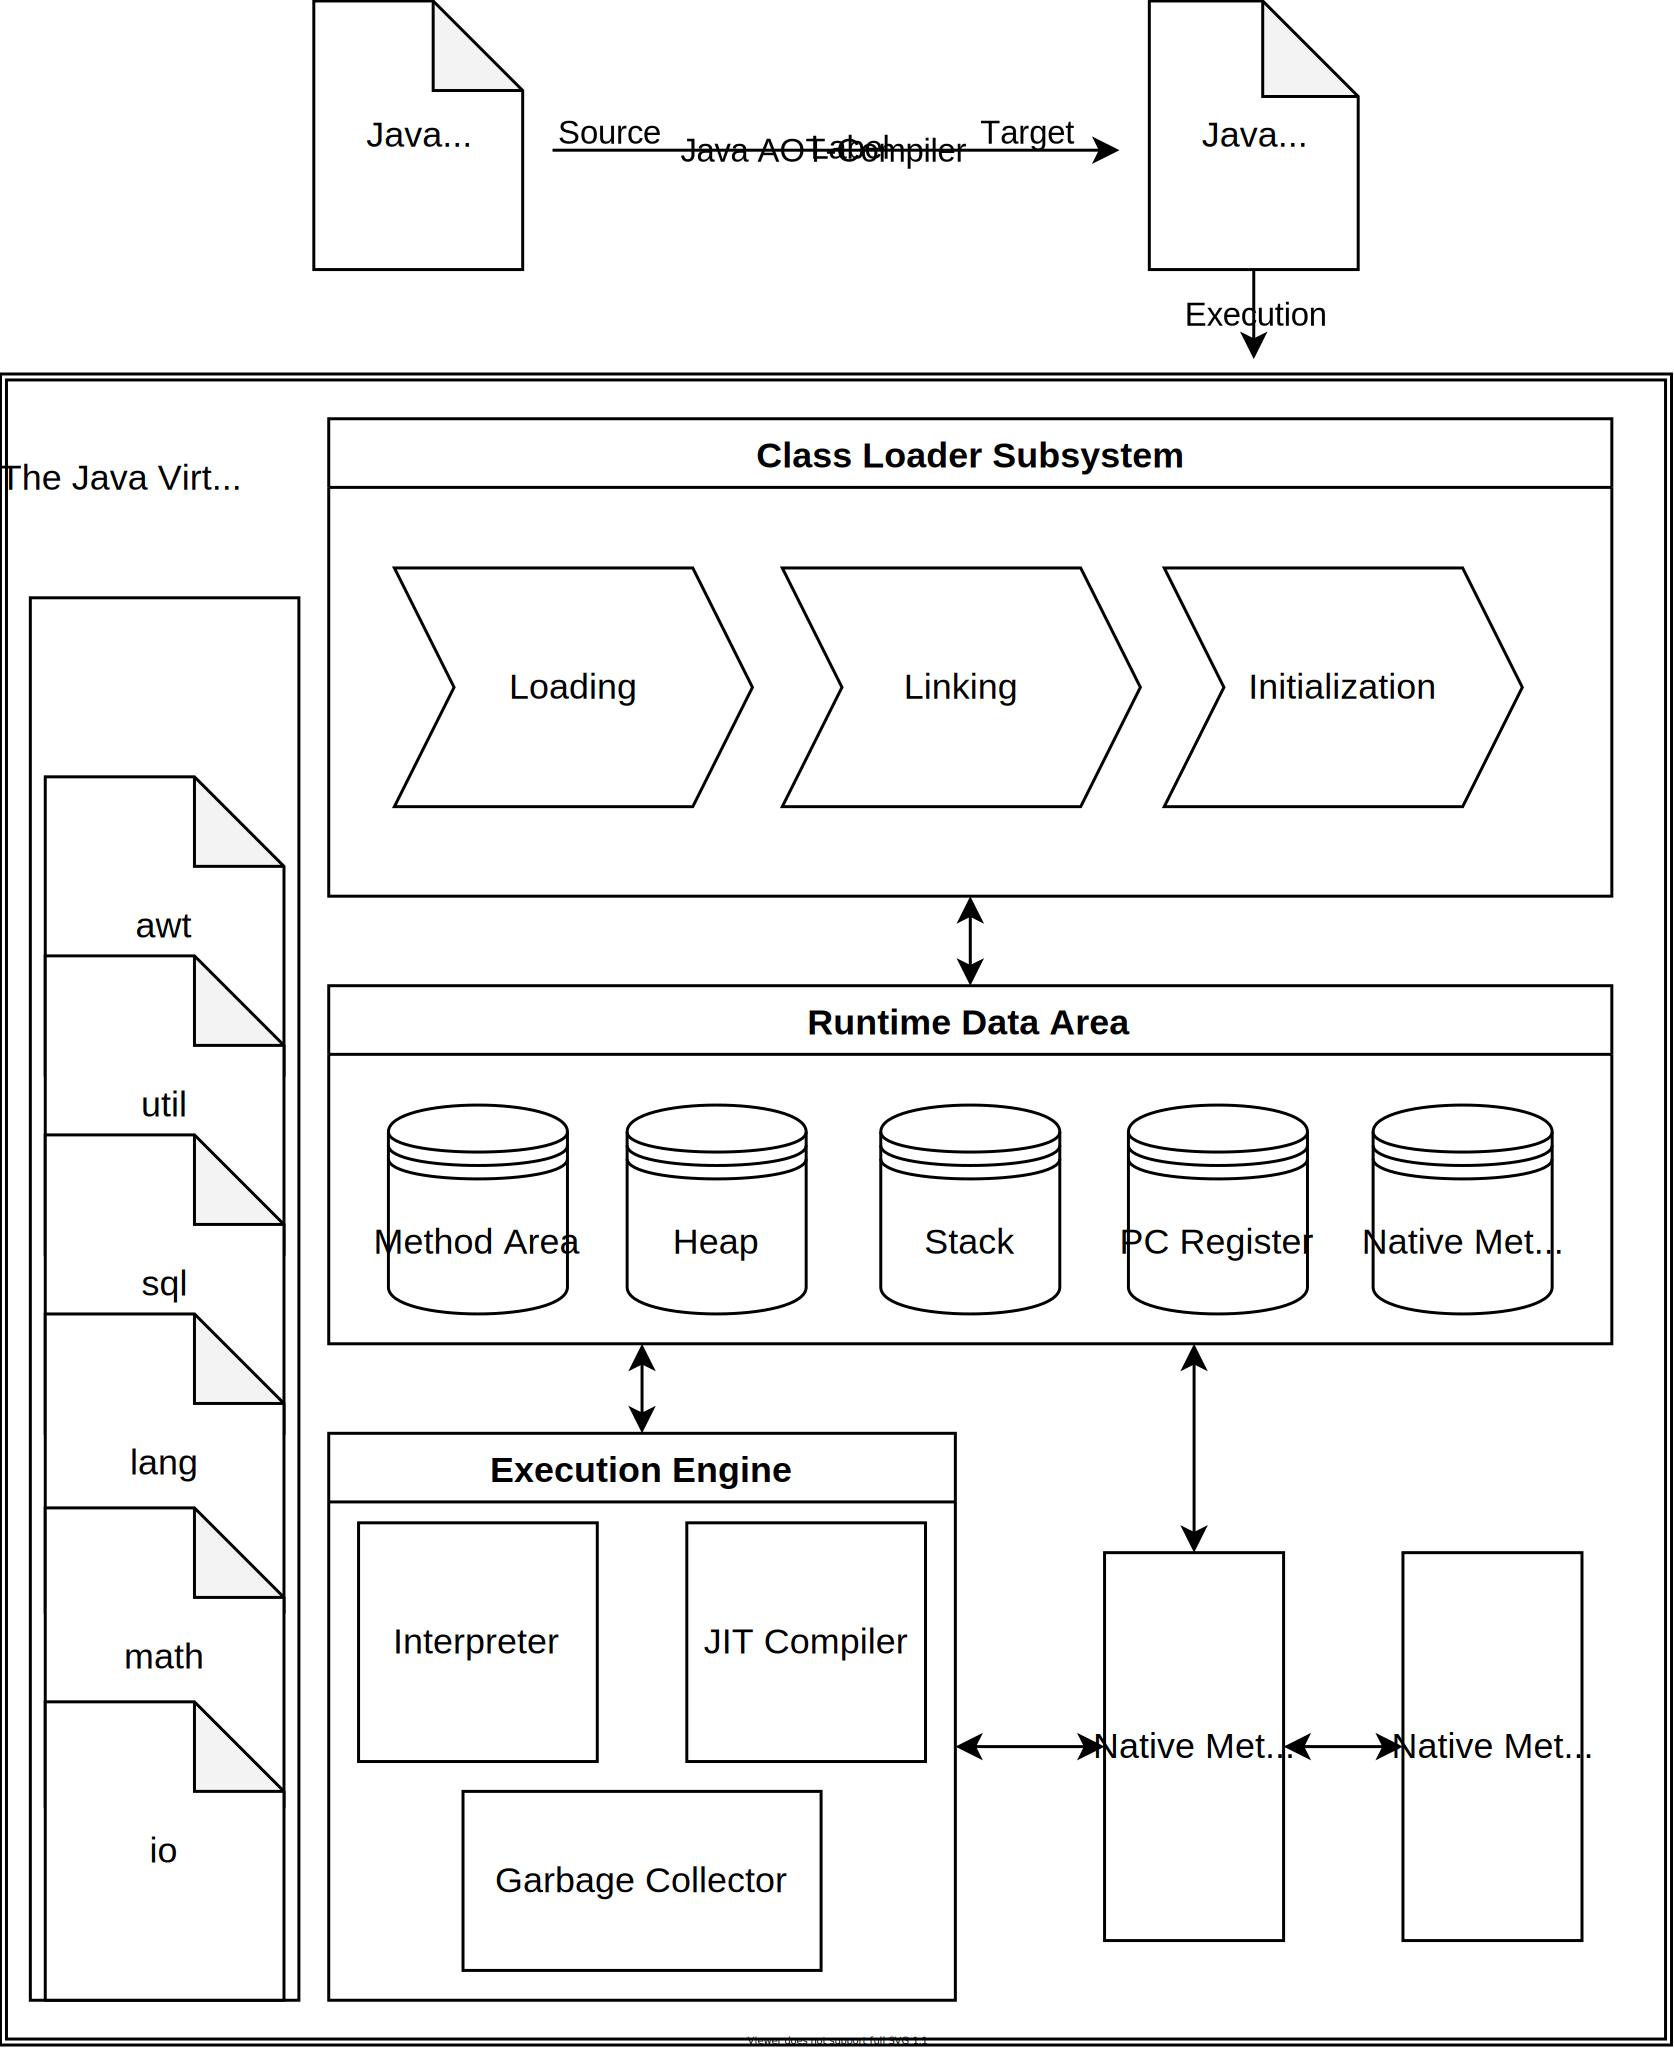
\includegraphics[scale=0.2]{../figures/JVM.png}
	\caption{The Java Virtual Machine simplified structure}
	\label{fig:jvm}
\end{figure}
When talking about the JVM the mentioning of classes and interfaces is inevitable.
In further parts the distinction between class and interface is abbreviated as class.
Multiple causes for class creation exist. The class to be created can be referenced by the constant pool of another class or a class' method can be invoked via reflection.\\
The creation at the start of a program works via loading the initial class and initializing it and furthermore invoking the specified method \emph{static void main(args[])}. The complete execution is driven by this method which, as soon as the program has more than this specific method and starting class, causes loading, linking and initialization of additional classes and invoking additional methods. How do the three steps, loading, linking and initialization work? The next paragraph talks about the beginning of a class creation and loading.\\
When creating a class in execution the JVM transforms the implementation-independent bytecode into an implementation-specific internal representation of the class. The algorithm is executed step by step meaning that a class has to be completely loaded before linking can be started and it has to be verified and prepared to the full extant before initialization.\\
The loading is started by the class loader which can be the JVM bootstrap loader or a user-defined one. Before the JVM starts the class loader it checks whether the pair binary class name and class loader already exist in which case the class already exists thus eliminating the necessity of class creation. If creation proves necessary the class loader has to find the class' bytecode representation on the specific platform, usually a file with the class' name in a hierarchical filesystem. After finding, if not a specific error is thrown, the JVM parses the bytecode, which in turn might not be valid resulting in different kinds of errors. Optional superclasses may also be resolved. After these steps the pair of loader and class are saved by the JVM. Loading usually concerns the class itself however linking concerns the whole ecosystem of the respective class. \\
The JVM links a class by preparing the class, superclasses, element type in case of array classes and resolving all symbolic references which as it is a recursive algorithm includes loading and linking these as well. The two strategies for resolution are an eager algorithm, meaning immediate loading and linking on verification, or loading and linking in a lazy way meaning resources are only loaded and linked when they are about to be used. At this point the JVM knows where the binary representation of a class can be found and which other classes are in the direct ecosystem of the class but the class' structure hasn't been checked yet.\\
Checking the class' structure is the main concern of the verification phase. In this step the class is checked for a static and structural constraints list. These include checks for appropriate type usage, number of arguments, instance initialization before usage, return types and many more. Any caught error in this step lead to ta thrown VerifyError. If no such error occurs the verification is finished and acknowledges the structual correctness of the binary class representation.\\
When doing the preparation of a class the JVM checks loading constraints on methods overriding those of superclasses and create and initialize static fields to default values. This phase can occur any time between creation and initializiation but imperatively before initialization.\\
Beforehand the resolution step with two different strategies has been discussed briefly without going into detail. This omission will be rectified now. Resolution in the context of the JVM means the process of dynamically determining conrete values from symbolic references in the run-time constant pool. The target of resolution includes classes, fields, methods, method types, method handles or dynamically computed constants. These different targets require different approaches. These usually require class loading, lookup, etc. They can also fail and throw errors or succeed resulting in a resolved dynamic binding in the constant pool. With all these preceding steps the class is now ready for initialization.\\
Conceptually initializing a class is fairly simple as it is the mere execution of the initialization method. This can only be invoked by certain cases or instructions like \emph{new} or a subclass is initialized resulting in the initialization of the superclass. At this point the JVMs multithreading needs to be taken in account since synchronization is imperative. This again is solely handled by the JVM and of no concern of the application programmer. The concrete inner workings are generally spoken handled by object states and unique initialization locks. The Initialization phase is the final stage of the class loader subsystem. Now the different data areas are explained briefly.\\
The JVM run-time data area is subdivided into five different data areas. These fulfill different tasks and are also different in their relation towards processes and threads as there are data areas being defined per thread and others per process. This results in some data areas existing as long as the JVM is running and some areas' existence is linked to their respective thread's existence. The data areas are, as can be seen in figure \ref{fig:jvm}, the method area, heap, stack, program counter register and the native method stack. The next paragraphs explain which area is responsible for which task and when they are created and destroyed.\\
The method area is shared between all JVM threads and is created on JVM start-up. It stores all per-class structures like the constant pool or field and method data.
The heap 
The stack is a thread-defined structure and is itself subdivided into thread-specific stacks. Regarding the data a stack holds: local variables, partial results and has its share in method invocation and return. The not necessarily contiguous stack is only changed by pushing and popping frames.
The program counter (PC) register holds the current program counters of all running threads. These PCs contain the address of the currently executed method.
The native method stack
With the dara areas explained the execution engine is the focus of the next few paragraphs.\\
The execution engine is mainly built up of three different components, the interpreter, the just-in-time (JIT) compiler and the garbage collector.\\
The interpreter is the part that executes the code directly/live including byte code getting translated to actual implementation-dependent machine code and its execution. When doing so the interpreter profiles the run code by keeping track for example of how often a certain piece of code is executed. This profiling information is then used to choose the parts of code that get jit-compiled

\cite{Lindholm}


\section{GraalVM}

\section{Truffle API}

\section{Graal.Js}

\section{ECMAScript modules}
\subsection{Current State}

\subsection{Proposal: Module blocks}

\chapter{Implementation}

This chapter lays out the implementation by presenting an architectural overview on how and where the proposal can be included in the Graal.js project. This inclusion is further detailed in the upcoming sections. The implementation explanation is then wrapped up by explaining the interaction with dynamic imports and the serialization / deserialization framework.

\section{General overview}
Before thinking about implementing the proposal in the Graal.js project one needs to know how source code is evaluated by Graal.js. The path of source code going through the engine is straightforward. Without going too deep into the specifics it follows Figure \ref{fig:mainImpl}. The source code is traversed and transformed into a token stream. This token stream is then evaluated by the parser which uses the identified tokens in conjunction with the specified grammar given by ECMAScript \cite{ecma} to transform them into an intermediate tree form. This tree contains nodes representing general language concepts without specifying the nodes into specialized forms. As can be seen in Figure \ref{fig:mainImpl} a module block is represented by a function node in the intermediate form. Later on in the translation pipeline the \texttt{GraalJSTranslator} class is called with an intermediate form node and translates it into a specified module block node. In the scope of this thesis a \texttt{FunctionNode} to a \texttt{ModuleBlockNode}. These specialized nodes are then executed when being visited in the tree. On the specifics of interpretation and compilation during execution see Section \ref{sec:graalcomp}. 

\begin{figure}[h!]
    \centering
    \includegraphics[scale=0.165]{figures/implMain.png}
    \caption{Code evaluation by Graal.js}
    \label{fig:mainImpl}
\end{figure}

Implementing the module block proposal into the Graal.js project involves several steps. Those are adjustments to the parser to capture the newly introduced syntax, implementation of the prototype, introducing a new respective node for module blocks and lastly adjusting the node for dynamic import-calls. At this point the implementation is limited to the available specification of the proposal. The chapter's outline is firstly the module block direct implementation into the Graal.js project followed by explanations of some necessary adjustments for dynamic import-calls. The direct implementation part is split up in four parts: parser changes, module block node, constructor and the prototype.The specific parser changes are explained in the next section.

\section{Parser}
From the specification we can take away that \texttt{module} won't be introduced as a keyword in ECMAScript meaning during parsing the token "module" will be treated as an identifier. As both identifier and module blocks are classified as so called \texttt{PrimaryExpressions} the main change is happening in this explicit parser method inplace of the "ident"-Token branch. Like Listing \ref{lst:impl:minModule} shows \texttt{module} can still be used as identifier. Thus recognizing a module block needs a lookahead token and additionally satisfy the no line delimiter condition. This is done by first checking for the next token being a \texttt{\{} after a \texttt{module} identifier , changing from the "ident"-branch to the module block branch and then checking whether there is at least one line delimiter between the \texttt{module} and the \texttt{\{}. A line delimiter occurrence would result in a syntax error. Otherwise the parsing continues with capturing all statements inside the module block similar to a regular module and then putting the result into the same intermediate representation form a regular module would be put in. This caters to the notion of modules and module blocks acting similar in the language specification. The only relevant difference is the end of the parsing which is the end of file in the module case and a closing brace (\texttt{\}}) in the module block case. The next section talks about further steps that are taken during translation.

\begin{lstlisting}[caption={Minimal module identifier example in JavaScript}, label={lst:impl:minModule}]
    var module = 42;
    
    var moduleBlock = module { };
\end{lstlisting}

\section{ModuleBlockNode: Module Blocks' Truffle AST representative}

The Graal.js project includes a class called \texttt{GraalJsTranslator}. This class is responsible for translating the intermediate representation nodes into specialized ones for the resulting AST. During execution of this class the intermediate module block representative gets translated into a module block node. The node is built according to the provisional proposal's specification meaning the hidden properties are set as defined. At the current point the \texttt{hostInitializeModuleBlock}-method which is mentioned in the specification is not implemented as it is not included in the specification yet. With the node representation itself finished the next section turns towards the prototype and the constructor.

\section{ModuleBlock prototype and constructor}

This part of the implementation is split up into two parts where firstly a discussion is depicted as to why the constructor is specified as is. Secondly the actual implementation is explained. At current state, as of July 2021, it is unwished for by the developers to implement yet another eval-esque structure coming from the desire for less dynamic evaluation. A point for including an actual constructor for module blocks would be the symmetry and consistency in the whole language's specification. This concern can be brought up since structures like \texttt{AsyncFunction} or \texttt{GeneratorFunction} do have constructors with a code-string parameter. Right now the eval-point outweighs the symmetry-/consistency-point. The constructor when called simply throws a type error. This concludes the rather simple implementation of the constructor with the discussion behind it maybe resulting in a change of the constructor's specification. The next paragraph concludes the implementation of the module block itself by introducing the module block prototype.

The prototype is constructed in a fairly simple way. Its prototype property is the module block Prototype Object with the general attributes writable, enumerable, and configurable all set to false as is standard in the ECMAScript specification. The module block Prototype Object is \\ \texttt{\%ModuleBlock.prototype\%}. Its internal prototype slot is \texttt{\%Object.prototype\%} and it is an ordinary Object. It has simply one function which is the toString() method. This method should check whether it is used on a \texttt{ModuleBlock} object and as such return the hidden \texttt{SourceText} property.
On a second note \texttt{ModuleBlock} is specified as global. This allows for the code in Listing \ref{fig:globModule} to work. Again this matter can be subject to change during the proposal's progress.

 \begin{lstlisting}[caption={ModuleBlock working as global in JavaScript}, label={fig:globModule}]
        var moduleBlock = module { };
        
        moduleBlock instanceof ModuleBlock; // true
\end{lstlisting}

This concludes the module block implementation itself. The module block's syntax is implemented in the parser, the module blocks runtime semantics are implemented in the specified module block node for the resulting AST and the constructor's and prototype's specification is met accordingly with also registering \texttt{ModuleBlock} as global. In conclusion the module block at this state is implemented as a standalone without much interaction with the rest of the EcmaScript ecosystem. This leads us to the question how does the module block interact with existing language features. The proposal's specification only states one interaction with another language feature: the import()-call. Thus the next paragraph states the necessary changes for integrating module blocks into the dynamic import calls.

\section{Interaction with dynamic import}

The interaction between module blocks and dynamic imports points to the Graal.js representative for dynamic imports, the class \texttt{ImportCallNode}. Hence, the class needs to be changed in this matter. The main difference is the change from using only Strings with the module's URL as identifiers to using the module block node as identifier for the resulting Module Record. To accomplish this, the object needs to be checked and if it does not satisfy the condition of being an object with the internal slot of \texttt{ModuleBlockBody}, a String is then used as identifier, otherwise the \texttt{ModuleBlockNode}. After that the regular \texttt{HostImportModuleDynamically} routine is called as would be for regular modules. This results in a Module Record which is saved in the module map. The module map itself also has to be changed to accept the module block node as key as well as the URLs used for regular modules. During that process the three-step phase of modules is executed. First the \texttt{ModuleBlock} source code gets parsed as it would be a separate module. It is then instantiated and at last evaluated. Through these explicit inner workings the module block preserves the positive effects of modules while eliminating the aforementioned negatives.

As mentioned above, dynamic imports is the only feature of the ECMAScript specification that interacts directly with module blocks. With the changes made on the \texttt{ImportCallNode} and the aforementioned changes to the parser, the introduction of the \texttt{ModuleBlockNode} and the registration of the respective prototype and constructor the implementation phase is finished. As already mentioned some specifics might have to be changed in the future as the proposal matures through the stages but the skeleton is laid out at this state. The following paragraph and Figure \ref{fig:blockVSmodule} conclude the implementation on a comparison between modules and module blocks on implementation level behavior.

\section{Serialization framework}

This section presents the framework for transferring module block source code from one process to another, i.e. one machine to another, potentially via network. This framework is not part of the module block proposal for ECMAScript, but a testing ground for the potential of the proposal. The goal is aimed for by implementing the framework is to offer code transfer over the network in a syntactically simple way. For this to be possible two builtin functions have to be implemented and registered at the \texttt{ModuleBlock} object in JavaScript. Their names exactly match their purpose: \texttt{serialize} and \texttt{deserialize}. The serialize method is straightforward and is oriented on the \texttt{toString}-method by accessing the \texttt{SourceText} property and then taking the string gained from the access and turning it into a String. This already concludes the serialization of a module block. The deserialization involves a few more steps. The given String has to be used to create an internal source object. Then the source code has to be parsed and translated as explained in Sections 3.2 and 3.3 to retrieve a \texttt{JSModuleRecord}. This record in turn is instantiated and evaluated and its resulting namespace is returned. The usage of the two builtin functions can be seen in Listing \ref{fig:globModuleAPI} where a module block is first created in Line 2, then serialized in Line 3, prepared for usage in a different module via deserialization in Line 8 and then gets used in Line 10.

 \begin{lstlisting}[caption={ModuleBlock serialization / deserialization}, label={fig:globModuleAPI}]
     // serialize module
    var moduleBlock = module { export var test = 5; };
    export var moduleBlock = ModuleBlock.prototype.serialize(moduleTest);
    
    // deserialize module
    import * as modules from 'moduleBlockSerializeModule.js';
    
    var tester = ModuleBlock.prototype.deserialize(modules.moduleBlock);
    
    vonsole.log(tester.test); // 5
\end{lstlisting} 

\section{Wrap up}

On regard of parsing the main difference between module blocks and modules is the outside call onto the class when parsing modules but module blocks have to be caught from inside the parser. Hence the parser is told explicitly to parse a module from another class while a module block is caught by the inner class's logic and will from then on be treated similarly to the regular module. Both parsing results are then encapsulated into the same intermediate representation as a \texttt{FunctionNode}. When translating this intermediate representation into the final AST representative the path of modules and module blocks splits up again as the module block is transformed into a \texttt{ModuleBlockNode} and the module is transformed into a \texttt{JSFunctionExpressionNode}. Finally as those constructs are imported, in the module's case also statically, dynamically the final result will always be a \texttt{JSModuleRecord} which is the AST's representation of the, in ECMAScript specified \cite{ecma}, Module Records. The description is also envisioned by the subsequent Figure \ref{fig:blockVSmodule} This brief difference in behavior explanation concludes the implementation chapter which is followed by the evaluation chapter detailing the testing of the, as set out above, implementation.

\begin{figure}[h!]
    \centering
    \includegraphics[scale=0.165]{figures/ModuleBlockVSModule.png}
    \caption{Simplified Graal.js translation pipeline of module blocks and modules}
    \label{fig:blockVSmodule}
\end{figure}

\chapter{Evaluation}

This chapter lays out the testing in two ways: functional and performance-wise. The functional tests include all relevant aspects of the specification being tested and the performance-wise tests conduct benchmarks with two different code examples.

\section{Functional testing}

The module blocks implementation as presented in Chapter 3 was evaluated by running the provided tests in the project. Those tests come from the Test262 implementation conformance test suite \cite{ecmaTest262}. Since these tests can't cover module block syntax and semantics additional tests were conducted.

The Test262 suite combines the three ecma standards ECMA-262 (ECMAScript Language Specification), ECMA-402 (ECMAScript Internationalization API Specification), and ECMA-404 (JSON Data Interchange Syntax / ISO/IEC 21778). The suite's test files cover any  behavior stated in these specifications and is comprised of more than 30.000 individual test files \cite{ecmaTest262, ecmaTestSpec}. Although the test environment is extensive full coverage cannot be guaranteed. It's certain to say that the suite doesn't yet contain any tests that cover module block functionality. This shifts the topic towards the tests that were designed and conducted in the course of this thesis.

The main orientation for designing tests regarding the module block proposal came from the available basic specification. While it is not finished yet, the parts of the specification that could be implemented can also be tested. First of, the syntactic part of the specification can already pose different testing scenarios.

    \begin{lstlisting}[caption={Module block syntax tests}, label={fig:testSyntax}]
        var module = 42;
        
        var nextModule = module;
        
        var moduleBlock = module { };
        
        var failingModuleBlock = module
            { };
    \end{lstlisting}

The first syntactic specialty is the fact that "module", while acting as a keyword in the scope of module blocks, won't be added to the keywords group in ECMAScript. The consequences are random variables being used with "module" as identifier are allowed and line delimiters between \texttt{module} and the \texttt{\{} are forbidden. Since the \texttt{ModuleBody} part of the module block syntax  is optional an empty module like in line three of Listing \ref{fig:testSyntax} is allowed. This concludes the three testing cases for the syntax. Next up are tests regarding the prototype and the constructor.

The constructor of module blocks basically doesn't have to exist as it simply should throw a \linebreak\texttt{TypeError}. The decision during implementation was made that it actually is implemented but when called throws the specified error. Still it doesn't change the expected behavior and thus a simple call to the constructor is made and expects the aforementioned error. Testing the prototype requires more elaborate testing since multiple aspects need to be checked. Those regard especially the prototype property of the module block prototype object itself but also the module block prototype property. The described tests are conducted by source code similar to Listing \ref{fig:testCoPro}.

    \begin{lstlisting}[caption={Module block constructor and prototype tests}, label={fig:testCoPro}]
        var constructorModuleBlock = new ModuleBlock(); // TypeError: ModuleBlock is not a constructor
        
        var moduleBlock = module { };
        
        var instanceTest = moduleBlock instanceof ModuleBlock; // true
        
        var moduleBlockPrototype = moduleBlock.constructor.prototype; // object
    \end{lstlisting}

The following tests mainly regard the module blocks interaction with different ECMAScript constructs inside of the module block, in particular the optional syntax part \texttt{ModuleBody}, and its interaction with the dynamic import. The interaction with existing ECMAScript structures is straightforward as all of them have to be used inside a module block as part of the \texttt{ModuleBody} to some extent. The following Listing \ref{fig:testGeneral} lists some example cases with a simple number variable, a function and an async function.

    \begin{lstlisting}[caption={Module block general test example cases}, label={fig:testGeneral}]
        var moduleBlock = module { export var x = 42; }; // export number
        
        var moduleBlockFunc = module { export function square(x) {
                return x * x;
            } 
        }; // export function
    
        var moduleBlockAsync = module {
            function resolve() {
                return new Promise(resolve => {
                        resolve('resolved inside module block')
                });
            }
        
            async function asyncCall() {
                return await resolve();
            }
        
            export var resolved = asyncCall(); 
        }; // export promise
    \end{lstlisting}

A particular case that should also be noted as it raised interest during the proposal presentation is the ability to bundle module imports into a module block which was also tested extensively with importing modules in the different possible ways and also importing module blocks. The specialties of module block imports are explained in the next bit.

Module blocks can only be imported dynamically with awaits. Since top level awaits are not supported dynamic imports have to be encapsulated in async functions. Hence imported module block module records are encapsulated in a promise and have to be processed in a \linebreak then-environment. Listing \ref{fig:testImp} shows the exact syntax needed for importing the module block as well as an example of the builtin toString function on line 4.

    \begin{lstlisting}[caption={Module block dynamic import test}, label={fig:testImp}]
        var test = (async function() {
            var moduleBlock = module { export var x = 42; }; // export number
            
            console.log(moduleBlock.toString()); //  module { export var x = 42; }
            
            return await import(moduleBlock);
        })();
        
        test.then( function(module) {
            console.log("Module block x: " + module.x);  // Module block x: 42
        });
    \end{lstlisting}

In conclusion adding a new feature into an engine for ECMAScript requires extensive testing. First off, the general preexisting test suite Test262 has to be applied to the changed semantics and the implementation has to pass the tests. Then, all intricacies of the proposal's specification have to be tested. Although the proposal is a rather syntactic one it still introduces semantics which have to be tested. Next up after all internals are checked the interaction with preexisting ECMAScript structures needs to take place which furthers the extensiveness of testing.

\section{Performance evaluation}

Runtime testing is required to examine the effect the implementation has on the execution time of code.  Although it is discredited to measure performance with so-called micro-benchmarks, it should be mentioned that the aspect of runtime testing in this specific scenario is the mere performance impact a module block call has versus regular function calls \cite{HennessyJohnL2007Ca:a}. Module block calls performance impact should be negligible in real world examples and thus it is more feasible to test examples explicitly tailored to this very feature. This will also be relevant for later stages when performance can be compared with other engines as soon as module blocks are implemented therein. This reasoning results in two rather simple benchmark tests.

The general framework takes source code written in JavaScript and creating a context. From the created context, the source is parsed and evaluated multiple times during a warm-up phase, in this case 20 runs. This phase serves the purpose of eliminating performance influence from engine startup amongst other influences. Then the same process, parsing and evaluating, is repeated a predefined amount of times while each run the time it takes is measured. Afterwards a statistical summary of the measured time is built and compared.

\subsection{Toy example}
The toy example is simple. The reference implementation consists merely of a function call returning \texttt{3+2}. The same goes for the module block implementation. Listing \ref{fig:Toy} shows the benchmark kernel. The module block exports \texttt{3} and when the promise of the module block is executed, the exported \texttt{3} is added \texttt{2}. The benchmark itself is programmed in Java, importing the JavaScript file and executing it inside a JVM by parsing and evaluating the code. Results show that there is no overhead coming from the module block call. In the contrary, the module block performs faster by a small margin. Figure \ref{fig:bToy} summarizes the results of 50 runs and shows that in comparison to the reference function call the module block implementation runs faster in general but has one outlier being the slowest run of all 100 runs combined.

\begin{lstlisting}[caption={Module block toy example}, label={fig:Toy}]
     var simple = (async function() {
        const moduleBlock = module { export var t = 3; };
        
        return await import(moduleBlock);
    })();
    
    simple.then(value => value.t+2);
    
    // java code loop
    // initial eval
    context.eval(mainSource);
    
    // warmup
    for (int i = 0; i < WARMUP; i++) {
        context.parse(mainSource);
        context.eval(mainSource);
    }
    
    // benchmark
    for (int i = 0; i < RUNS; i++) {
        startTime = System.nanoTime();
        
        context.parse(mainSource);
        context.eval(mainSource);
        
        endTime = System.nanoTime();
        
        durations[i] = (endTime - startTime) / TIME_CONVERSION;
    }
\end{lstlisting}

\begin{figure}[h!]
    \centering
    \includegraphics[scale=0.7]{figures/runtimesToyBoxplot.png}
    \caption{Benchmark boxplots for toy example}
    \label{fig:bToy}
\end{figure}

\subsection{k-means}
The second example implements a simple application of the k-means clustering algorithm.\footnote{The interested reader can find more information on the algorithm in the Journal of the Royal Statistical Society. Series C (Applied Statistics) Vol. 28, No. 1 (1979), pp. 100-108, or as a German source:  https://www-m9.ma.tum.de/material/felix-klein/clustering/Methoden/K-Means.php}
The general code setup for the module block example is shown in Listing \ref{fig:kMeans}. The module block contains all constants function declarations and calls necessary to perform a cluster calculation via the k-means algorithm. The module block then is embedded into a promise via a dynamic import. The benchmark used for the toy example is also used with the k-means algorithm. The results again show no noticeable performance overhead on the module block's part and thus recreate the findings of the toy example. Figure \ref{fig:bKMeans} summarizes the results of 50 runs and shows that in comparison to the reference runtime, function calls regularly and from module, show no better performance than the respective module block calls.

\begin{lstlisting}[caption={Module block toy example}, label={fig:kMeans}]
    // *.js module block code
    (async function() {
        var kMeans = module {
            const ...
            function() ...
            // kMeans magic
            createRandomData();
            cluster();
        };
        
        return await import(kMeans)
    })();
\end{lstlisting}

\begin{figure}[h!]
    \centering
    \includegraphics[scale=0.7]{figures/runtimesKMeansBoxplot.png}
    \caption{Benchmark boxplots for k-means example}
    \label{fig:bKMeans}
\end{figure}
\pagebreak
The benchmarks were conducted on a PC with Windows 10, an Intel 3700K i7 processor and 16 GB RAM. Overall it can be summarized that as the two examples show, no explicit performance loss due to module block calls can be noted. The only tendency, that can be noted, is the outliers in the module block cases. Module block code produces significantly more outliers and is thus not as reliable performance-wise as the regular function calls. 

\chapter{Future Work}

Future Work on the thesis's matter is tightly tied to progress on the module block proposal. At current state the proposal resides at stage two where neither the specification is finalized nor the details are all cleared. A specific case of this is the hostInitializeModuleBlock-method mentioned in the runtime semantics of the module block specification, as it is merely mentioned but not specified. The work needs to be continued to keep the implementation on par with the specification. Especially as soon as the proposal reaches stage three the final specification is available. Subsequently the implementation has to be adjusted to fit the final version. Furthermore as the proposal progresses official tests will be released and later on embedded into the official Test262 suite. Those tests then have to be applied to the finished implementation. The preceding development description is rather rough, therefore the following paragraphs discuss details on the proposal that are not fixed yet.

A controversial implementation detail up for possible change is the constructor of module blocks. At current development state a constructor call leads to a TypeError. The relevant point for rejecting the ability to create a module block via a constructor is that module blocks would turn into an eval-like structure which is unwanted for as the web community generally rejects the eval-method. Due to security issues this sentiment gained widespread support. On the other hand one can argue that a language's design should be sound and symmetrical. Other structures that were introduced in ECMAScript that share the eval-like constructor discussion do have a working constructor. Thus for reasons of symmetry module blocks should have a constructor as well. The result of the discussion will be visible latest at stage three of the proposal. Right now the simple constructor implementation only throws the error and would have to be fully implemented if a working constructor is introduced in the proposal.

Another feature that might be introduced is an abbriviated form of module blocks. Due to the feature's rather syntactic nature the requirement are parser changes leading then into the same semantics as module blocks. The feature might be included if import-free-single-function module blocks become a frequently recurring pattern. Also not entirely clear is what the import.meta.url of a module block should look like. Although it is save to assume that it's bound to the module's import.meta.url in which it is specified it is frowned upon to be the exact same. A possible setup would be the module's import.meta.url directly followed by something like: "$L\#^+C\#^+$" where the \#s stand for the exact line and column number of the module block. As this is also not fixed yet the implementation has to follow suit as soon as the import.meta.url semantics are fixed.

In short, the implementation cannot be finalized in the scope of the thesis as the proposal won't be finished by far. A lot of details need to be worked on before the proposal can reach stage three. With stage three reached the implementation can be finished as the specification will be finished more or less. The testing in the scope of the thesis has to be adapted to the final implementation and the tests being released before the proposal can reach stage four. Since the implementation is tied closely to the proposal it can only be done as soon as the proposal is completed and adopted by moving to stage 4 which will earliest be in 2022.



\chapter{Conclusions}

In the scope of the thesis the ECMAScript TC39 proposal "module blocks" was implemented into the Graal.js project which resides inside the GraalVM ecosystem. The implementation was split into a syntactic and semantic part, with the semantic part being conducted through introducing a new Node according to general Truffle rules and the given proposal specification. The syntactic part was introduced via minor changes in the preexisting Graal.js parser. Testing the implementation consisted of applying the preexisting Test262 official ECMAScript test suite and explicitly for the proposal written unit tests on it. To finish off embedding the proposal a serialization algorithm was written and tested with a proof of concept test via a Worker. Reiterating the fact that the proposal is not finished yet and supposed to undergo changes, it can be said that the base for contributing this stage two proposal to the Graal.js project is laid out.


%%%%%%%%%%%
\begin{singlespace}
	\listoffigures
    \lstlistoflistings
\end{singlespace}


\backmatter

\printbibliography

\appendix

\end{document}
